%:
% !TEX TS-program = pdflatex
% !TEX encoding = UTF-8 Unicode

% This is a simple template for a LaTeX document using the "article" class.
% See "book", "report", "letter" for other types of document.

\documentclass{report}
%\documentclass{scrartcl}
%\documentclass[11pt]{report} % use larger type; default would be 10pt
%\setkomafont{disposition}{\normalfont\bfseries}	

\usepackage[utf8]{inputenc} % set input encoding (not needed with XeLaTeX)

%%% PAGE DIMENSIONS
\usepackage{geometry} % to change the page dimensions
\usepackage{amsmath}
\geometry{a4paper} % or letterpaper (US) or a5paper or....
% \geometry{margin=2in} % for example, change the margins to 2 inches all round
% \geometry{landscape} % set up the page for landscape
%   read geometry.pdf for detailed page layout information

\usepackage{booktabs}% http://ctan.org/pkg/booktabs

\usepackage{graphicx} % support the \includegraphics command and options
\usepackage{natbib} % support the \includegraphics command and options
\usepackage{xcolor,colortbl}

\usepackage{multicol}

% \usepackage[parfill]{parskip} % Activate to begin paragraphs with an empty line rather than an indent

%%% PACKAGES
\usepackage{booktabs} % for much better looking tables
\usepackage{array} % for better arrays (eg matrices) in maths
\usepackage{paralist} % very flexible & customisable lists (eg. enumerate/itemize, etc.)
\usepackage{verbatim} % adds environment for commenting out blocks of text & for better verbatim
\usepackage{subfigure} % make it possible to include more than one captioned figure/table in a single float
% These packages are all incorporated in the memoir class to one degree or another...

%%% HEADERS & FOOTERS
\usepackage{fancyhdr} % This should be set AFTER setting up the page geometry
\pagestyle{fancy} % options: empty , plain , fancy
\renewcommand{\headrulewidth}{0pt} % customise the layout...
\lhead{}\chead{}\rhead{}
\lfoot{}\cfoot{\thepage}\rfoot{}

%%% SECTION TITLE APPEARANCE
\usepackage{sectsty}
\allsectionsfont{\sffamily\mdseries\upshape} % (See the fntguide.pdf for font help)
% (This matches ConTeXt defaults)

%%% ToC (table of contents) APPEARANCE
\usepackage[nottoc,notlof,notlot]{tocbibind} % Put the bibliography in the ToC
\usepackage[titles,subfigure]{tocloft} % Alter the style of the Table of Contents
\renewcommand{\cftsecfont}{\rmfamily\mdseries\upshape}
\renewcommand{\cftsecpagefont}{\rmfamily\mdseries\upshape} % No bold!

\usepackage{titling}
\usepackage[brazil]{babel}
\usepackage{xspace}

\usepackage{framed}

\usepackage{setspace}
\onehalfspacing

\usepackage{url}

%\DeclareUnicodeCharacter{00A0}{ }

%%% END Article customizations

%%% The "real" document content comes below...

\begin{document}

\pagestyle{empty} % Removes page numbers

\newcommand{\sw}{\textit{software}\xspace}
\newcommand{\Sw}{\textit{Software}\xspace}
\newcommand{\sws}{\textit{softwares}\xspace}
\newcommand{\iso}{ISO 29110\xspace}
\newcommand{\dsw}{Desenvolvimento de \Sw}

\newcommand{\gp}{Gerente de Projeto\xspace}
\newcommand{\kick}{reunião de \textit{kick-off} do projeto\xspace}
\newcommand{\Kick}{Reunião de \textit{kick-off} do projeto\xspace}
\newcommand{\stake}{\textit{stakeholders}\xspace}
\newcommand{\bline}{\textit{baseline}\xspace}

\newcommand{\amb}{Fatores ambientais da empresa\xspace}
\newcommand{\ativ}{Ativos de processos organizacionais\xspace}

% nomenclaturas de documentação
\newcommand{\planproj}{Plano de Gerenciamento do Projeto\xspace}
\newcommand{\planesc}{Plano de Gerenciamento do Escopo\xspace}
\newcommand{\plancron}{Plano de Gerenciamento do Cronograma\xspace}
\newcommand{\plancusto}{Plano de Gerenciamento de Custos\xspace}
\newcommand{\planqual}{Plano de Gerenciamento da Qualidade\xspace}
\newcommand{\planpess}{Plano de Gerenciamento de Pessoal\xspace}
\newcommand{\plancom}{Plano de Gerenciamento das Comunicações\xspace}
\newcommand{\planrisco}{Plano de Gerenciamento de Riscos\xspace}
\newcommand{\planaq}{Plano de Gerenciamento de Aquisições\xspace}

\newcommand{\termo}{Termo de Abertura do Projeto\xspace}

\newcommand{\bok}{Guia PMBOK$^{\small{\textregistered}}$\xspace}

\newcommand{\pmi}{PMI$^{\small{\textregistered}}$\xspace}

\newcommand{\msp}{Project\xspace}

% schedule forecast
\newcommand{\schfor}{Previsão de cronograma\xspace}
\newcommand{\costfor}{Previsão de custos\xspace}

%\renewcommand{\chapter}{\section}

\newcommand*{\plogo}{\fbox{$\mathcal{PL}$}} % Generic publisher logo

%----------------------------------------------------------------------------------------
%	TITLE PAGE
%----------------------------------------------------------------------------------------

\newcommand*{\titleGP}{\begingroup % Create the command for including the title page in the document
	\centering % Center all text
	\vspace*{\baselineskip} % White space at the top of the page
	
	\rule{\textwidth}{1.6pt}\vspace*{-\baselineskip}\vspace*{2pt} % Thick horizontal line
	\rule{\textwidth}{0.4pt}\\[\baselineskip] % Thin horizontal line

{\Huge Apostila de Gestão de Projetos \\[0.5\baselineskip]  ~Gerenciamento do escopo do projeto}\\[0.2\baselineskip] 

%	{\LARGE \\
%		 }\\[0.2\baselineskip] % Title
	
	\rule{\textwidth}{0.4pt}\vspace*{-\baselineskip}\vspace{3.2pt} % Thin horizontal line
	\rule{\textwidth}{1.6pt}\\[\baselineskip] % Thick horizontal line
	
%	\scshape % Small caps
%	A number of fascinating and life-changing templates \\ % Tagline(s) or further description
%	presented  in a clear and useable way \\[\baselineskip] % Tagline(s) or further description
	\bok e \pmi são marcas registradas do Project Management Institute, Inc.\par % Location and year
	
	\vspace*{2\baselineskip} % Whitespace between location/year and editors
	
	Editado por \\[\baselineskip]
	{\Large Gladistone M. Afonso\par} % Editor list
%	{\itshape The University of California \\ Berkeley\par} % Editor affiliation
	
	\vfill % Whitespace between editor names and publisher logo
	
%	\plogo \\[0.3\baselineskip] % Publisher logo
	{\scshape 2015} \\[0.3\baselineskip] % Year published
	{\large Curso de extensão em Gestão de Projetos\\FASE/FMP}\par % Publisher
	
	\endgroup}

%----------------------------------------------------------------------------------------
%	BLANK DOCUMENT
%----------------------------------------------------------------------------------------

%\begin{document} 
	
%	\pagestyle{empty} % Removes page numbers
	
%	\titleGP % This command includes the title page
	
%\end{document}


%\title{Apostila de Gestão de Projetos\\Gerenciamento de Integracao}
%%\title{Area de conhecimento do \bok \citep{pmbok}}.
%\author{Gladistone M. Afonso}
%
%\date{}
%\maketitle
%\newpage

\titleGP % This command includes the title page

% !TEX root = Apostila GP.tex

\chapter{Gerenciamento do Escopo}

\section{O que é escopo}

Segundo \cite{pmbok}, escopo  é  todo  o  trabalho,  e  somente  o  trabalho  necessário  para  que  o  produto  ou 
serviço objetivo do projeto seja entregue ao seu final.

Esse é o \textbf{Escopo do projeto} que não deve ser confundido com o \textbf{Escopo do produto}, que são os atributos, funcionalidades e características que devem estar presentes no produto ou serviço criado pelo projeto, conforme podemos observar na Figura \ref{fig:escopo:proj:prod}.

\begin{figure}[!h]
\centering
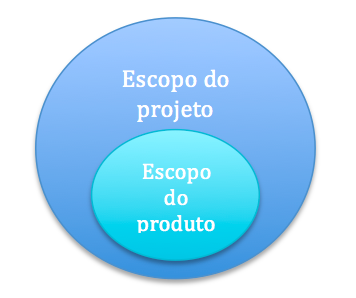
\includegraphics[scale=0.5]{Figuras/escopo_proj_prod.png}
\caption{Escopo produto X escopo projeto}
\label{fig:escopo:proj:prod}
\end{figure}

\section{Gerenciamento do Escopo}

Sãos os processos que visam garantir que o projeto inclua todo o trabalho necessários para completar com sucesso o projeto.

Para isso, deve incluir:

\begin{itemize}

\item Definir e controlar o que \textbf{faz} e o que \textbf{não faz} parte do projeto.

\item Controlar se todo o trabalho está sendo realizado.

\item Controlar o processo de mudanças do escopo.

\item Confrontar as mudanças com o \termo.

\item Evitar retrabalho ou trabalho desnecessário e seus custos

\end{itemize}

\section{Processos}

Para garantir a gerência do escopo, são necessários os seguintes processos:

\begin{itemize}

\item \textbf{Coleta de requisitos}: definir e documentar o que é necessário para se alcançar os objetivos do projeto.

\item \textbf{Definição do escopo}: descrição detalhada do projeto e do produto.

\item \textbf{Criação da Estrutura Analítica do Projeto (EAP)}: a fim de facilitar o gerenciamento das entregas e do trabalho, o escopo deve ser dividido em partes menores e estruturadas.

\item \textbf{Verificação do escopo}: formalizar a aceitação das entregas finalizadas do projeto.

\item \textbf{Controle do escopo}: monitorar e gerenciar o andamento e as mudanças na linha de base do escopo.

\end{itemize}

Os processos dentro do ciclo de vida do projeto podem ser observados na Figura \ref{fig:ciclo:vida}.

\begin{figure}[!h]
\centering
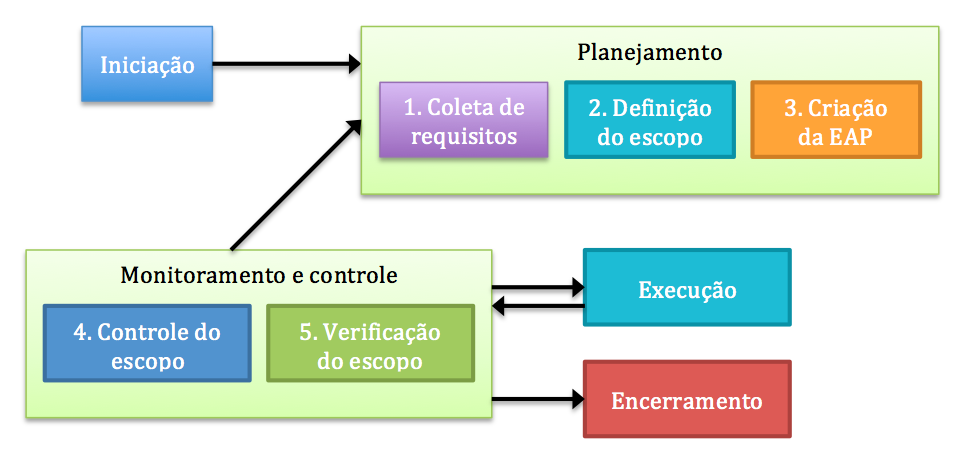
\includegraphics[scale=0.5]{Figuras/ciclo_vida.png}
\caption{Processos dentro do ciclo de vida do projeto}
\label{fig:ciclo:vida}
\end{figure}

\subsection{Inimigos do escopo}

Um escopo com problemas pode levar o projeto ao seu fim. Por isso é importante observar os dois principais inimigos do escopo:

\begin{itemize}

\item \textbf{\textit{Scope Creep}}: aumento do escopo sem nenhum controle, de maneira contínua, muitas vezes de forma lenta, que resulta em um escopo ``inchado'', ingerenciável, cujo foco foge da ideia inicial do projeto e o resultado reflete no aumento dos custos e perda de prazos.

\item \textbf{\textit{Gold Plating}}: adicionar elementos não especificados nos requisitos do projeto, geralmente partindo de equipes técnicas e de desenvolvimento sob a alegação de agregar valor mas cujo resultado é o aumento de custos, perda de qualidade e aumento desnecessário da complexidade do produto.

\end{itemize}

\subsection{Requisitos}

São condições ou capacidades que devem ser supridas pelo resultado do projeto (produto ou serviço) a fim de satisfazer um contrato ou outro documento formal.

São dividos em:

\begin{itemize}

\item \textbf{Requisitos funcionais:} o que o produto ou serviço deve \textbf{fazer}.

\item \textbf{Requisitos não-funcionais:} o que o produto ou serviço deve \textbf{ter}.

\end{itemize}


%\bibliographystyle{plain}
%\bibliographystyle{bibstyle/latex8}     
%\bibliographystyle{apalike-url}     


\bibliographystyle{Bibliografia/apalike-pt}     

%\bibliographystyle{lastchecked}     
            
\bibliography{Bibliografia/research}

\end{document}